%TODO: CORREGIR COMANDOS PARA QUE SE VEAN CON VERB
%TODO: INTENTAR QUITAR LA MORRAYA QUE NO SIRVA
%TODO: INTENTAR NO REPETIR TANTAS COSAS EN EL EJERCICIO 3
%TODO: REVISAR DOCUMENTO PARA FALLOS ORTOGRAFICOS/GRAMATICALES
\documentclass{article}
\usepackage[utf8]{inputenc}
\usepackage[spanish]{babel}
\usepackage{graphicx, graphics, float, hyperref}
\usepackage{listings}
\usepackage[a4paper, total={6in, 10in}]{geometry}

\title{SSO Práctica 2 Sesión 1}
\author{Andrés Merlo Trujillo}
\date{}
\hypersetup{
    colorlinks=true,
    linkcolor=black,
}

\begin{document}

\maketitle

\tableofcontents

\newpage
%\addcontentsline{toc}{section}{Ejercicio 1}
%\section*{Ejercicio 1}
%\begin{figure}[H]
%    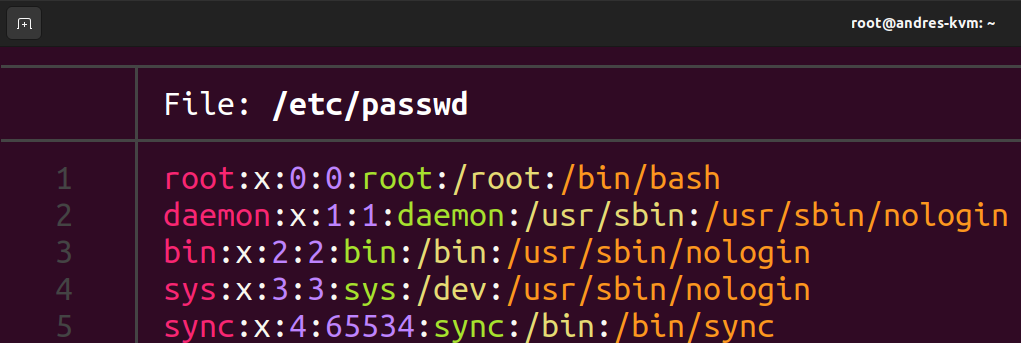
\includegraphics[width=\textwidth]{imagenes/passwdfile.png}
%    \caption{Ejemplo de entradas en el archivo.}
%\end{figure}

\addcontentsline{toc}{section}{Ejercicio 1}
\section*{Ejercicio 1}

Para ello voy a crear los siguientes programas:

%foto programa C++

%foto programa C

Y voy a usar las siguientes ordenes para compilarlos:

\verb|g++ -o salidaCPP holaMundo.cpp|
\verb|gcc -o salidaC holaMundo.c|


\addcontentsline{toc}{subsection}{Apartado A}
\subsection*{Apartado A}
A continuacion explicaré que contiene cada seccion, para obtener informacion se puede usar la orden \verb|man 5 elf|:

\begin{itemize}
    \item \textbf{.interp}: Esta seccion almacena la ruta del interprete del programa. Si el archvo tiene un segmento que incluye esta seccion, los atributos de la seccion tendran el bit SHF\_ALLOC. La seccion es de tipo SHT\_PROGBITS.
    
    \item \textbf{.got}: Esta seccion almacena la tabla de desplazamientos global (Global Offset Table). Es de tipo SH\_PROGBITS y sus atributos son especificos del procesador. 
    
    \item \textbf{.got.plt}: Esta seccion almacena la tabla de vinculacion de procedimientos (Procedure Linkage Table). Es de tipo SH\_PROGBITS y sus atributos son especificos del procesador. Sirve para obtener las direcciones a funciones para posteriormente poder ser llamadas.
\end{itemize}


\addcontentsline{toc}{subsection}{Apartado B}
\subsection*{Apartado B}

Ejecutando la orden \verb|readelf -S ejecutable| podemos obtener las secciones que componen el programa.

%foto de cpp con readelf

%foto de c con readelf

Ahora, para mostrar por terminal la diferencia de los archivos a color se puede usar la orden \verb|icdiff archivo1 archivo2|.

%foto de icdiff (quizas haya que cortarlas)

Como se puede ver, en la primera linea, el offset es distinto, siendo mas alto en el programa escrito en C++. Ademas, se puede ver que algunas secciones del programa escrito en C++ son ligeramente mas grandes que la version en C. Las secciones afectadas son: .gun.hash, .dynsym, .dynstr, .gun.version, .rela.dyn, .rela.plt, .plt, .plt.sec, .text, .eh\_frame\_hdr, .eh\_frame, .init\_array, .fini\_array, .dynamic, .got, .bss, .symtab, y .strtab.

Por ultimo, tambien se puede ver que el desplazamiento (offset) y las direcciones de memoria de estas secciones varia entre una version y otra.


\bigskip

Las secciones .ctors y .dtors contienen lo siguiente:

\begin{itemize}
    \item \textbf{.ctors}: Esta seccion almacena punteros inicializados a las funciones del constructor de C++ (constructores de las clases).
    \item \textbf{.dtors}: Esta seccion almacena punteros inicializados a las funciones del destructor de C++ (destructores de las clases).
\end{itemize}


\addcontentsline{toc}{subsection}{Apartado C}
\subsection*{Apartado C}

Mediante la orden \verb|readelf -r programa| podemos ver las distintas secciones que contiene. Estas son:

\begin{itemize}
    \item \textbf{.rela.dyn}: Contiene las entradas de reubicacion para simbolos dinamicos; es decir, estas variables deben ser reubicadas en tiempo de ejecucion.
    \item \textbf{.rela.plt}: Contiene las entradas de reubicacion para simbolos de funciones. Al igual que el anterior, deben ser reubicadas en tiempo de ejecucion.
\end{itemize}

Ademas, la version de C++ tiene mas entradas que la version de C, como pasó en el apartado anterior.


\addcontentsline{toc}{section}{Ejercicio 2}
\section*{Ejercicio 2}


\addcontentsline{toc}{subsection}{Apartado A}
\subsection*{Apartado A}

El ocmando \verb|objdump| tiene algunos switches similares a los de \verb|readelf|. A continuacion voy a indicar algunos que se han usado en el ejercicio anterior:

\begin{itemize}
    \item \verb|readelf -r <archivo>| $\rightarrow$ \verb|objdump -Rr <archivo>|
    
    
    Muestra las entradas de reubicacion del archivo ELF.

    %foto readelf y objdump side by side


    \item \verb|readelf -h <archivo>| $\rightarrow$ \verb|objdump -f <archivo>|
    
    Muestra las cabeceras del propio archivo ELF.

    %foto side by side

    \item \verb|readelf -S <archivo>| $\rightarrow$ \verb|objdump -h <archivo>|
    
    Muestra la informacion de las cabeceras de seccion (section headers).

    %foto side by side

    \item \verb|readelf -l <archivo>| $\rightarrow$ \verb|objdump -p <archivo>|
    
    Muestra las cabeceras del programa.

    %foto side by side

\end{itemize}

% TABLE: READELF VS OBJDUMP
% -r / -Rr
% -h / -f
% -S / -h
% -l / -p

\addcontentsline{toc}{subsection}{Apartado B}
\subsection*{Apartado B}

Esta herramienta sirve de mucha utilidad desde el punto de ingenieria inversa, ya que permite el desensamblado de un ejecutable en las instrucciones maquina que lo compone.

%foto de eso
%caption: salida producida por el comando ``objdump -d salidaC'', se puede ver la seccion main en <_start>

Esto simplifica mucho el trabajo, ya que no es necesario buscar en lois manuales de los procesadores que instruccion tiene cada codigo. Ademas, esto permite buscar vulnerabilidades en el programa o incluso el estudio de las distintas condiciones para que continue el codigo para luego poder intentar saltarse las medidas de seguridad.


\addcontentsline{toc}{section}{Ejercicio 3}
\section*{Ejercicio 3}

He realizado la siguiente modificacion al prorgama en su version C:

%modificacion del rpograma con sleep

%Y para la version en C++ tambien he realizado lo mismo:

%modificacion del rpograma con sleep

Ahora, mediante el simbolo ``\&'' se puede ejecutar el programa en segundo plano. A continuacion, se busca el proceso pasando la salida de la orden \verb|ps -e| mediante un pipe a la orden \verb|grep|. Por tanto, en mi caso, la orden para encontrar el PID del programa seria asi: \verb|ps -e | | \verb|grep hola|.

%salida de ps

Y sabiendo que tiene el PID 18770, con cualquier orden para mostrar texto como \verb|nano, cat, bat| se puede ver lo que contieene.

%salida de proc pid maps

Ahora, con la orden \verb|readelf -S <archivo>| podemos ver las secciones que componen el ejecutable:

%foto de la salida

Usando la orden \verb|readelf -Wl <archivo>| se pueden obtener las cabeceras del programa.

%foto


El kernel cuando ve INTERP, carga el primer LOAD, despues los segmentos del prorgama interprete y finalemnte se cargan las bibliotecas especificadas en LD\_PRELOAD y los segmentos DYNAMIC. Estos segemntos que se cargan se pueden ver con la orden \verb|readelf -d <archivo>|.

%foto de la salida

\end{document}
